\section{Problem 3.2}

Given a Z channel with probabilities $p_{Y|X}(0|0)=1$, $p_{Y|X}(1|0)=0$, $p_{Y|X}(1|1)=p_{Y|X}(0|1)=\frac{1}{2}$, we want to find the channel capacity $C$. We know that the channel capacity for a discrete memory channel is defined as follows.

\begin{equation}
	C = \max_{p_X} I(X;Y) = H(Y)-H(Y|X)
\end{equation}

First we compute the value of $H(Y)$ and $H(Y|X)$ in function of $p_X$.

\begin{align*}
	H(Y)= & -Prob\{y=1\}\cdot\log(Prob\{y=1\})-Prob\{y=0\}\cdot\log(Prob\{y=0\}) \\
	= & -p_{Y|X}(1|1) \cdot p_X(1) \cdot\log(p_{Y|X}(1|1) \cdot p_X(1)) \\ & -(p_{Y|X}(0|0) \cdot p_X(0) + p_{Y|X}(0|1) \cdot p_X(1)) \cdot\log(p_{Y|X}(0|0) \cdot p_X(0) + p_{Y|X}(0|1) \cdot p_X(1)) \\
	= & -\frac{1}{2}\cdot p_X(1)\log\Big(\frac{1}{2}\cdot p_X(1)\Big)-\Big(p_X(0)+\frac{1}{2}\cdot p_X(1)\Big)\cdot \log \Big(p_X(0)+\frac{1}{2}\cdot p_X(1)\Big) \\
	= & -\frac{1}{2}\cdot p_X(1)\log\Big(\frac{1}{2}\cdot p_X(1)\Big)-\Big(1-\frac{1}{2}\cdot p_X(1)\Big)\cdot \log \Big(1-\frac{1}{2}\cdot p_X(1)\Big)
\end{align*}

\begin{figure}[h]
	\centering
	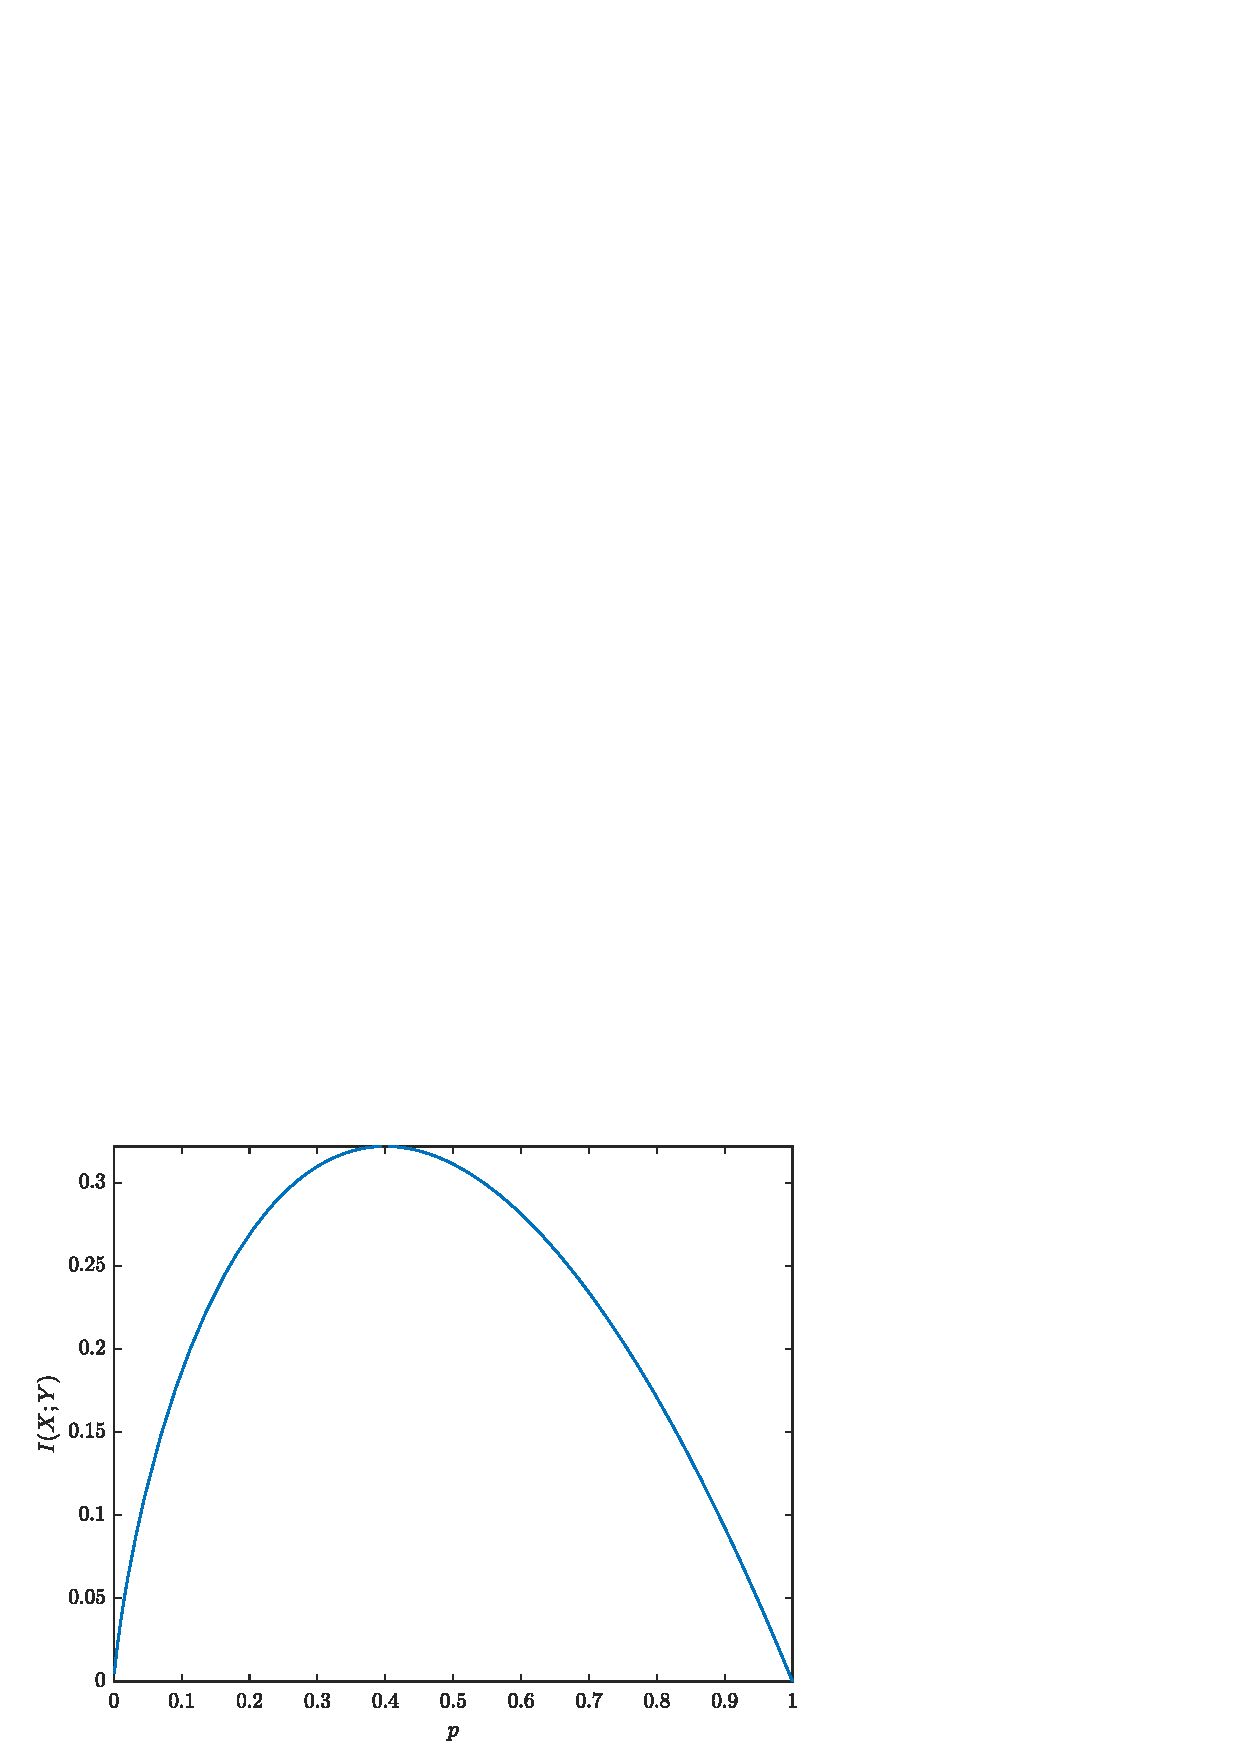
\includegraphics[width=0.7\linewidth]{img/func_info_ex1}
	\caption{Mutual information as a function of $p \triangleq p_X(1)$}
	\label{fig:funcinfoex1}
\end{figure}
